\pagenumbering{arabic} % Evita duplicados en numeración
\cleardoublepage

% ============================
% SECCIÓN: ESTRUCTURA GENERAL DE UN CAPÍTULO 
 %(sección 6 en config.tex)
%=================
\chapter{Capitulo}
\fancyhead{} % Borra el encabezado
\thispagestyle{fancy}

Texto...Texto...Texto...Texto...Texto...Texto...Texto...Texto...Texto...

Texto...Texto...Texto...Texto...Texto...Texto...Texto...Texto...Texto...
\section{Seccion} 
Texto...Texto...Texto...Texto...Texto...Texto...Texto...Texto...Texto...

Texto...Texto...Texto...Texto...Texto...Texto...Texto...Texto...Texto...
\subsection{Subseccion}
Texto...Texto...Texto...Texto...Texto...Texto...Texto...Texto...Texto...

Texto...Texto...Texto...Texto...Texto...Texto...Texto...Texto...Texto...
\subsubsection{Subsubsection}

\paragraph{Parrafo}
Texto...Texto...Texto...Texto...Texto...Texto...Texto...Texto...Texto...

Texto...Texto...Texto...Texto...Texto...Texto...Texto...Texto...Texto...
\subparagraph{Subparrafo}
Texto...Texto...Texto...Texto...Texto...Texto...Texto...Texto...Texto...

Texto...Texto...Texto...Texto...Texto...Texto...Texto...Texto...Texto...


 % ======== 
 % Solution
 \begin{activity}[Trabaja en parejas]
  Encuentra tres ejemplos de grupos que no sean abelianos.
\end{activity}

\begin{definition}[Este término es clave]
  Un \emph{grupo} es un conjunto con una operación binaria que satisface la asociatividad, tiene un elemento neutro y cada elemento posee un inverso.
\end{definition}

\begin{example}[Grupo simple]
  El conjunto de los enteros \( \mathbb{Z} \) con la suma es un grupo.
\end{example}

\begin{exercise}[Intenta resolverlo]
  Demuestra que el conjunto de los enteros pares forma un subgrupo de \( \mathbb{Z} \).
\end{exercise}

\begin{generality}[Por qué importa la generalidad]
  El concepto de grupo abstrae la idea de simetría, aplicable en álgebra, geometría y física.
\end{generality}

\begin{note}[Consejo sobre notación]
  El elemento neutro suele denotarse por \( e \) o \( 1 \), según el contexto.
\end{note}

\begin{property}[Clausura]
  El producto de dos elementos cualesquiera de un grupo pertenece también al grupo.
\end{property}

\begin{remark}[Confusión común]
  Recuerda: la operación del grupo no tiene que ser multiplicación.
\end{remark}

\begin{solution}[prueba de conteo]
  La derivada de \( f(x) = x^2 \) es \( f'(x) = 2x \).
  Aplicamos la regla de la potencia para obtener este resultado.
\end{solution}

\begin{summary}[Ideas clave del capítulo]
  Este capítulo abordó la definición formal de grupo, ejemplos importantes como \((\mathbb{Z}, +)\), y propiedades clave como la existencia del neutro e inverso.
\end{summary}

\begin{theorem}[Propiedad básica de los grupos]
  Si \( G \) es un grupo y \( a, b \in G \), entonces \( ab^{-1} \in G \).
\end{theorem}

\begin{warnbox}[Precaución al usar propiedades conmutativas]
  No todas las operaciones son conmutativas. Asegúrate de verificar las propiedades antes de aplicarlas.
\end{warnbox}
    
%===========================================================
 \section{Entornos predefinidos} 
 
  quote	      Sangrado especial
  quotation	  Similar a quote
  verse	      Para poesía (maneja saltos de línea)
  center	    Centra texto
  flushleft	  Alinea a la izquierda
  flushright	Alinea a la derecha
  itemize	    Lista con viñetas
  enumerate	  Lista numerada
  description	Lista con etiquetas personalizadas
 

\section{Jerarquía de secciones}

Los comandos de jerarquía de secciones son utiles para generar el índice y agregar "títulos". 

\begin{center}
  \begin{tabular}{|c|l|c|}
  \hline
  \textbf{Nivel} & \textbf{Etiqueta} & \textbf{Disponible en} \\
  \hline
  0 & \verb|\part| & \verb|book| o \verb|report| \\
  1 & \verb|\chapter| & \verb|book| o \verb|report| \\
  2 & \verb|\section| & Todas las clases \\
  3 & \verb|\subsection| & Todas las clases \\
  4 & \verb|\subsubsection| & Todas las clases \\
  5 & \verb|\paragraph| & Todas las clases \\
  6 & \verb|\subparagraph| & Todas las clases \\
  \hline
  \end{tabular}
  \end{center}

Sin embargo, \textbf{no están pensadas para ser usadas como simples contenedores de texto}.  
Si se desea escribir párrafos de texto normales, lo correcto es usar líneas en blanco entre bloques de texto en vez de estas.

\begin{custompar}
  Si se desea escribir párrafos con formato personalizado, lo recomendable es definir un entorno personalizado usando 
  \textbf{\texttt{\textbackslash newenvironment}} en el archivo de configuración (sección 6 en este proyecto,tambien se puede modificar el formato del texto general).
  \end{custompar}

% ============================
%  Alineaciones de párrafos: 
 
 \textbf{Alineaciones de párrafos}

 \begin{flushleft}
 Este párrafo estará alineado a la izquierda.
 \end{flushleft}
 
 \begin{center}
 Este párrafo estará centrado.
 \end{center}
 
 \begin{flushright}
 Este párrafo estará alineado a la derecha.
 \end{flushright}
 
% ============================
%  Texto con marcos 
 
\textbf{Texto con marcos}
 
 % Requiere: \usepackage{framed}
 \begin{framed}
 Este párrafo está dentro de un marco.
 \end{framed}
 
 % Requiere: \usepackage{mdframed}
 \begin{mdframed}
 Este párrafo está dentro de un marco con más opciones de estilo.
 \end{mdframed}
 
 \clearpage
% ============================
% SECCIÓN: EJEMPLO LISTAS
 %(seccion 14 en config.tex)
 
 \section{Ejemplo de listas}
 
  \subsection{Lista estandar}
   Ejemplo \texttt{Titulo de la lista}:


  
  \subsection{Lista con titulos definidos}
   \begin{description}
      \item[Contexto:] Comprender el contexto histórico del tema.
      \item[Problema:] Identificar los problemas clave a resolver.
      \item[Revisión:] Revisar trabajos previos relevantes.
    \end{description}
    
    \clearpage
% ============================
% SECCIÓN: EJEMPLO DE CITAS Y BIBLIOGRAFIA
 % (seccion 12 en config.tex)
 % Requisitos (ya estan implementados):
 %  
 % 1-Cargar el archivo .bib en  main.tex (Justo despues de \documentclass) 
 % 2-Definir la cita en el archivo .bib (En /tex/Material_de_referencia)
 % 3-Imprimir la bibliografia con \printbibliography (Esta al final del main.tex)
 \section{Ejemplo de citas}
 
 % Cómo citar en LaTeX (bibliografía .bib)

 Este es un ejemplo de cita de un libro: \cite{EjemploLibro}.  
 Se usa para referirse a libros, artículos, documentación, etc.
 
 % Archivo .bib obligatorio
 Las citas deben estar definidas en un archivo \textbf{bib.}  
 En este proyecto
 
 % Mostrar bibliografía al final
 El comando \texttt{\textbf{printbibliography}} imprime solo las fuentes citadas en el documento.  
Se coloca normalmente en las últimas partes del documento, como en \texttt{\textbf{main.tex}}.

El comando \texttt{\textbf{nocite\{*\}}} fuerza a incluir todas las entradas del archivo \texttt{\textbf{.bib}}, incluso si no fueron citadas.
 % Ejemplo de cita textual corta
 \begin{quote}
 Esta es una cita corta. Se muestra con márgenes más estrechos.
 \end{quote}
 
 % Ejemplo de cita textual larga
 \begin{quotation}
 Esta es una cita más larga.
 
 Puede contener varios párrafos.
 \end{quotation}
 \clearpage
% ============================
%  SECCIÓN: EJEMPLO NOTAS AL PIE Y REFERENCIAS
 %(seccion 12 en config.tex)
 
 \section{Ejemplo de notas al pie de página y referencias cruzadas}

 Este ejemplo muestra cómo crear referencias cruzadas y notas al pie de página en \LaTeX.
 
 Para crear una referencia cruzada, utiliza el comando \textbf{\texttt{\textbackslash label\{etiqueta\}}}
 para asignar una etiqueta a una sección. Luego, usa \textbf{\texttt{\textbackslash ref\{etiqueta\}}} o 
 \textbf{\texttt{\textbackslash autoref\{etiqueta\}}} para referenciarla en otra parte del documento.
 
 Para agregar una nota al pie, utiliza \textbf{\texttt{\textbackslash footnote\{texto de la nota\}}}.
 
 

\footnote{Coloca el comando justo donde deseas que aparezca el número de la nota al pie.}
 
 \subsection{Sección de ejemplo} 

 \label{sec:ejemplo}% Lleva a lo que este abajo de la etiqueta
 Esta sección de ejemplo es referenciada con \texttt{\textbackslash label\{etiqueta\}}.


 Texto...Texto...Texto...Texto...Texto...Texto...Texto...Texto...Texto...

 Texto...Texto...Texto...Texto...Texto...Texto...Texto...Texto...Texto...

 Texto...Texto...Texto...Texto...Texto...Texto...Texto...Texto...Texto...

 Referencia al apendice A \autoref{sec:Apendice A}

 \subsection{Referencia cruzada} 
 Para más información, consulta la \autoref{sec:ejemplo}, que contiene detalles sobre cómo usar notas al pie 
 y referencias cruzadas.
 En esta parte vamos a poner la nota a pie de pagina\footnote{Ejemplo nota al pie de pagina}
 
 las notas tambien pueden tener referencias\footnote{\autoref{sec:ejemplo}}

 \clearpage 
% ============================
%  SECCIÓN: EJEMPLO GLOSARIOS, ABREVIACIONES, SIGLAS Y SIMBOLOS 
 %  (sección 11 en config.tex)
 %  Las entradas se cargan desde un archivo externo (17-glossary.tex)
 %  Se incluye en main.tex con: 
 %     \input{tex/03-Material_de_referencia/17-glossary.tex}
 
 \section{Ejemplo de uso de glosarios definidos}

 \textbf{Los glosarios se imprimen al final del documento*}
 Después de la primera mención de un acrónimo,
 las siguientes veces que uses la misma etiqueta mostrará la forma abreviada. 
 % ============================
 \subsection{Glosario de términos generales}
 
 % Las entradas definidas con \newglossaryentry sin "type=" van al glosario principal.
 
 En este caso la abreviacion siempre se muestra corta:
 algoritmo abreviacion = \gls{algoritmo} 
 si se define se puede usar una forma plural =  \glspl{algoritmo}  
 otro  ejemplo mal definido = \gls{modelo} 
 
 % ============================
 \subsection{Lista de abreviaciones y siglas}
 
 Las siglas definidas con newacronym se imprimen completas la primera vez, luego abreviadas.
 
 La \gls{cpu} realiza las tareas básicas de procesamiento.  
 Una \gls{gpu} moderna puede acelerar algoritmos complejos.
 Por su parte, la \gls{gpu} es más eficiente para el procesamiento gráfico intensivo.  
 
 % ============================
 \subsection{Glosario de símbolos}
  
 % Entradas definidas con type=symbols. El nombre puede tener notación matemática.
 Para usar  un glosario personalizado hay que definir el glosario en el preambulo de tu main 

 El símbolo \gls{alpha} representa el coeficiente de expansión térmica.  
 La \gls{lambda} indica la longitud de onda en fenómenos ondulatorios.
 
 \subsection{Ejemplo de uso de glosarios personalizados}
 
 La constante de Planck, representada por \gls{planck}, es fundamental en la teoría cuántica.  
 La constante de gravitación universal, denotada por \gls{gravitacional}, juega un papel crucial en la física gravitacional.

 \clearpage 
% ============================
%  SECCIÓN: EJEMPLO FIGURAS Y TABLAS
 %(seccion 9 en config.tex)

 \clearpage % Fuerza salto de página para procesar cualquier figura/tabla pendiente
 \section{Figuras y tablas}

 Este capítulo ofrece ejemplos prácticos de cómo trabajar con tablas y figuras en \LaTeX.
 
 % ----------------------------
 % SUBSECCIÓN: TABLAS
 % ----------------------------
  
  \subsection{Tablas en \LaTeX}
  
  \begin{table}[H] % [H] del paquete float obliga a poner la tabla exactamente aquí
      \centering
      \begin{tabular}{|c|c|c|} % Tres columnas centradas con bordes verticales
          \hline
          \textbf{ID} & \textbf{Nombre} & \textbf{Edad} \\
          \hline
          1 & Juan Pérez  & 30 \\
          2 & María López & 25 \\
          3 & Luis García & 35 \\
          \hline
      \end{tabular}
      \caption{Ejemplo de tabla creada con \LaTeX.}
      \label{tab:ejemplo_tabla}
  \end{table}
  
 % Usando booktabs
 \subsubsection{Usando booktabs}

 \begin{table}[H]
   \centering
   \begin{tabular}{ccc}
     \toprule
     ID & Nombre & Edad \\
     \midrule
     1 & Juan Pérez  & 30 \\
     2 & María López & 25 \\
     3 & Luis García & 35 \\
     \bottomrule
   \end{tabular}
   \caption{Tabla con estilo \texttt{booktabs}.}
   \label{tab:booktabs}
 \end{table}
 
  \subsubsection{Consejos sobre tablas}
  Si las tablas son simples, se pueden escribir directamente como en el ejemplo anterior.  
  Para tablas extensas que ocupen varias páginas, se recomienda usar el paquete `longtable` o `tabu`.
 
 % ----------------------------
 % SUBSECCIÓN: FIGURAS
 % ----------------------------
  
  \subsection{Figuras en \LaTeX}
  
  Ejemplo de cómo insertar imágenes externas:
  
  \begin{figure}[H]
      \centering
      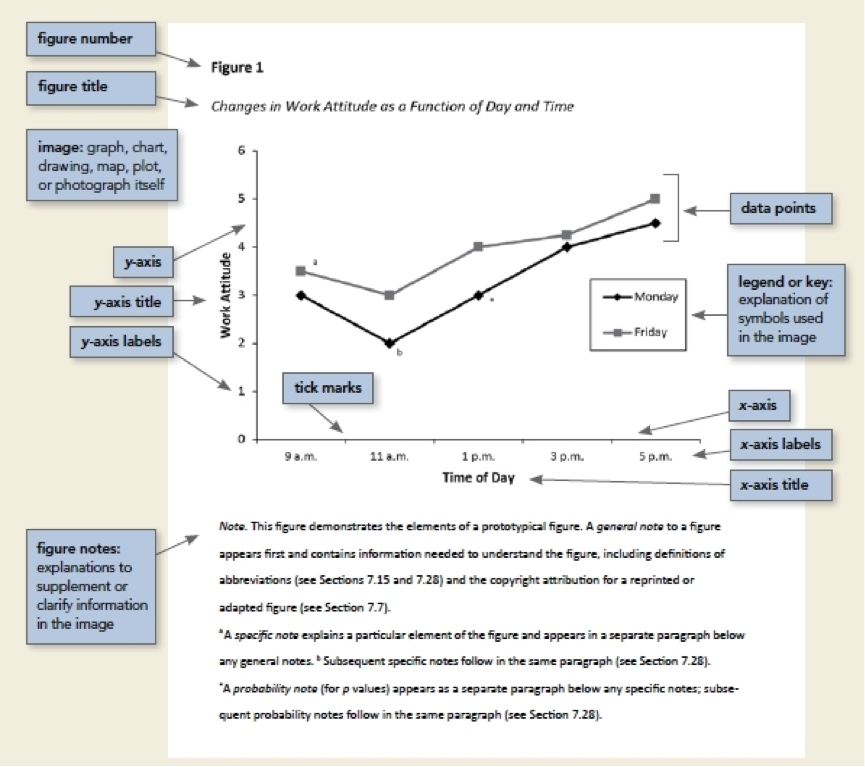
\includegraphics[width=0.7\textwidth]{images/figura.png}
      \caption{Ejemplo de figura externa representada como una imagen.}
      \label{fig:ejemplo_figura}
  \end{figure}
  
  \subsubsection{Consejos sobre figuras}
  Para diagramas, gráficas o ilustraciones técnicas, es preferible usar herramientas como `TikZ` o `PGFPlots` en lugar de imágenes externas.  
  Esto mantiene consistencia tipográfica, escalabilidad y edición directa desde el código fuente.
  
 
\clearpage 